%
% - - - - - - - xFitter discussion from Keping, Nov. 19 2019.
%
\section{Hessian profiling of the ATLAS 7 TeV $W/Z$ Data}
\label{sec:Appendix4xFitter}


{\bf The $\chi^{2}$ definitions in \texttt{xFitter} and \texttt{ePump}.}
%
As an alternative to directly including new data inside a full QCD global fit, Hessian PDF-profiling techniques provide a fast and flexible approach to explore the
impact of new data on a given PDF set; these profiling methods are available within both the \texttt{xFitter} and \texttt{ePump} frameworks.
In \texttt{xFitter}, the $\chi^{2}$ function includes both experimental and theoretical uncertainties \cite{Paukkunen:2014zia,Camarda:2015zba,xFmanual}:	
%
\begin{equation}\label{eq:chi2xfitter}
\chi^{2}(\vec{\lambda}_{\textrm{exp}},\vec{\lambda}_{\textrm{th}})=
\sum_{i=1}^{N_{pt}}\frac{\left[D_{i}+\sum_{\alpha}\beta^{\textrm{exp}}_{i,\alpha}\lambda_{\alpha,\textrm{exp}}-
T_i-\sum_{\alpha}\beta_{i,\alpha}^{\textrm{th}}\lambda_{\alpha,\textrm{th}}
\right]^{2}}{s_{i}^{2}}+\sum_{\alpha}\lambda_{\alpha,\textrm{exp}}^{2}+\sum_{\alpha}T^2\lambda_{\alpha,\textrm{th}}^{2}.
\end{equation}
%
Here $D_{i}$ and $T_i$ are the $i$-th experimental datum and corresponding theoretical prediction, respectively, where the index $i$ runs over all $N_\mathit{pt}$ points in a given experiment. 
%
Meanwhile, $s_{i}$ denotes the total uncorrelated uncertainty, $\beta_{i,\alpha}^{\textrm{exp}}\, (\beta_{i,\alpha}^{\textrm{th}})$ represents the correlated experimental (theoretical) uncertainties,
and $\lambda_{\alpha,\textrm{exp}}\, (\lambda_{\alpha,\textrm{th}})$ are the corresponding nuisance parameters. In this case, the index $\alpha$ runs over the $N_\lambda$ correlated systematic
uncertainties in an experiment, or over the $N_\mathit{ev}$ Hessian eigenvector directions of the PDF error sets. Theoretical uncertainties are determined according to predictions
based upon the corresponding PDF error sets, $f_\alpha^\pm$, as
%
\begin{equation}
\beta_{i,\alpha}^{\textrm{th}}=\frac{T_i(f_{\alpha}^{+})-T_i(f_{\alpha}^{-})}{2},
\end{equation}
%
in which $f_{\alpha}^{\pm}$ are the PDF error sets corresponding to positive and negative variations along eigenvector $\alpha$. The tolerance parameter $T$ is set to 1 or 1.645 if the PDF error sets are defined at the 68\% or 90\% C.L., respectively. Instead of scaling down the theoretical uncertainties $\beta^{\textrm{th}}_{i,\alpha}$ as in Ref.~\cite{xFmanual}, we equivalently scale up the corresponding nuisance parameters $\lambda_{\alpha,\textrm{th}}$ in order to compare with \texttt{ePump} \cite{Schmidt:2018hvu,Hou:2019gfw} more transparently.

The $\chi^{2}$ function in Eq.~(\ref{eq:chi2xfitter}) can be converted into the form defined in \texttt{ePump} \cite{Schmidt:2018hvu,Hou:2019gfw}:
%
\begin{equation}\label{eq:chi2ePump}
\Delta\chi^{2}(\vec{\lambda}_{\textrm{th}})
=\sum_{i,j=1}^{N_\mathit{pt}}
[D_i-T_{i}(\vec{\lambda}_{\textrm{th}})]
\textrm{cov}_{ij}^{-1}[D_j-T_{j}(\vec{\lambda}_{\textrm{th}})]
+\sum_{\alpha}T^2\lambda_{\alpha,\textrm{th}}^{2},
\end{equation}
%
where $\textrm{cov}_{ij}^{-1}$ is the inverse experimental covariance matrix constructed from $s_i$ and
$\beta_{i,\alpha}^{\textrm{exp}}$ \cite{Gao:2013xoa}. 
%With the tolerance being set to $T$ =1(1.645) for the 68\%(90\%) C.L. PDF error sets, Eq. (\ref{eq:chi2ePump}) becomes identical to Eq. (\ref{eq:chi2xfitter}). 
More generally, \texttt{ePump} also contains the option of the so-called ``dynamical tolerance'' $T^{(\alpha)}$ \cite{Schmidt:2018hvu,Hou:2019gfw}, whose specific value can be dependent on the corresponding PDF eigenvector direction, for the purpose of capturing the additional constraints to determine the PDF error sets, such as Tier-2 penalty used in the CT PDFs ~\cite{Dulat:2015mca}. The minimum of the $\chi^{2}$
function quantifies the compatibility between theory and data, and the minimization of $\chi^{2}$ optimizes the PDFs to describe the data \cite{Paukkunen:2014zia,Schmidt:2018hvu}.
In the linear approximation, the ``updated'' (or, in the language of \texttt{xFitter}, the ``profiled'') central PDF set, $f_{0}^{'}$, can be given in terms of nuisance parameters,
$\lambda_{\alpha,\textrm{th}}^{\textrm{min}}$, at the $\chi^{2}$ minimum:
%
\begin{equation}\label{eq:updatePDF}
f_{0}'=f_{0}+\sum_{\alpha} \lambda^{\textrm{min}}_{\alpha,\textrm{th}}\frac{f_{\alpha}^{+}-f_{\alpha}^{-}}{2}.
\end{equation}
%
The \texttt{xFitter}-profiled PDFs also include second-order diagonal terms, \linebreak
$\sim\! \frac{1}{2}(\lambda^{\textrm{min}}_{\alpha,\textrm{th}})^{2}(f_\alpha^{+}+f_\alpha^{-}-2f_0)$.
We note that the off-diagonal terms, $\sim\! \lambda^{\textrm{min}}_{\alpha,\textrm{th}}\lambda^{\textrm{min}}_{\alpha^\prime,\textrm{th}}$ for $\alpha\neq \alpha^\prime$, are not presently included,
since the off-diagonal, second-order partial derivatives cannot be constructed solely in terms of Hessian PDF error sets \cite{Hou:2016sho}. 
 
 
 \begin{table}
\centering
\caption{The $\chi^2$ values for the ATLAS 7 TeV $W/Z$ data before and after \texttt{xFitter} profiling and \texttt{ePump} updating, using the CT14 and CT18 PDFs. 
%We do not update  CT18A(Z) fits to avoid doubly counting the impact of ATL7ZW data.
}
\label{tab:chi2}
\begin{tabular}{c||c|c||c|c|c}
\hline\hline
Program & \multicolumn{2}{c||}{\texttt{xFitter}} & \multicolumn{3}{c}{\texttt{ePump}} \\
\hline
 PDFs & input & profiled & input & 
 $\begin{array}{c}
 \mbox{updated with}\\
 T^2=1.645^2,\\ 
 \mbox{as in \texttt{xFitter}}
 \end{array}
 $& 
 $\begin{array}{c}
 \mbox{updated with}\\
 \mbox{dynamical tolerance,}\\ 
 \mbox{as in CT18 fit}
 \end{array}
 $
 \\
\hline
\multicolumn{6}{c}{All the 7 measurements, $N_{\textrm{pt}}=61$}\\
\hline
CT14     & 290 & 106  & 285  & 104  &197  \\
CT18     & 362 & 104  & 356  & 103 &  199   \\
%CT18A   & 142 & --  & 140  & --  & --\\
%CT18Z   & 142 &  -- & 142  &  -- & --\\
\hline
\multicolumn{6}{c}{$W^{+},W^{-}$, $Z$-peak DY (central), $N_{\textrm{pt}}=34$}\\
\hline
CT14     & 224 & 66  & 220  &  66  & 140\\
CT18     & 294 & 63 & 289  &  63 &  144\\
%CT18A   & 87 & --  & 87   & -- & --\\
%CT18Z   & 88 & --  & 88  & --  & --\\
\hline
\hline
\end{tabular}
\end{table}

\begin{figure}
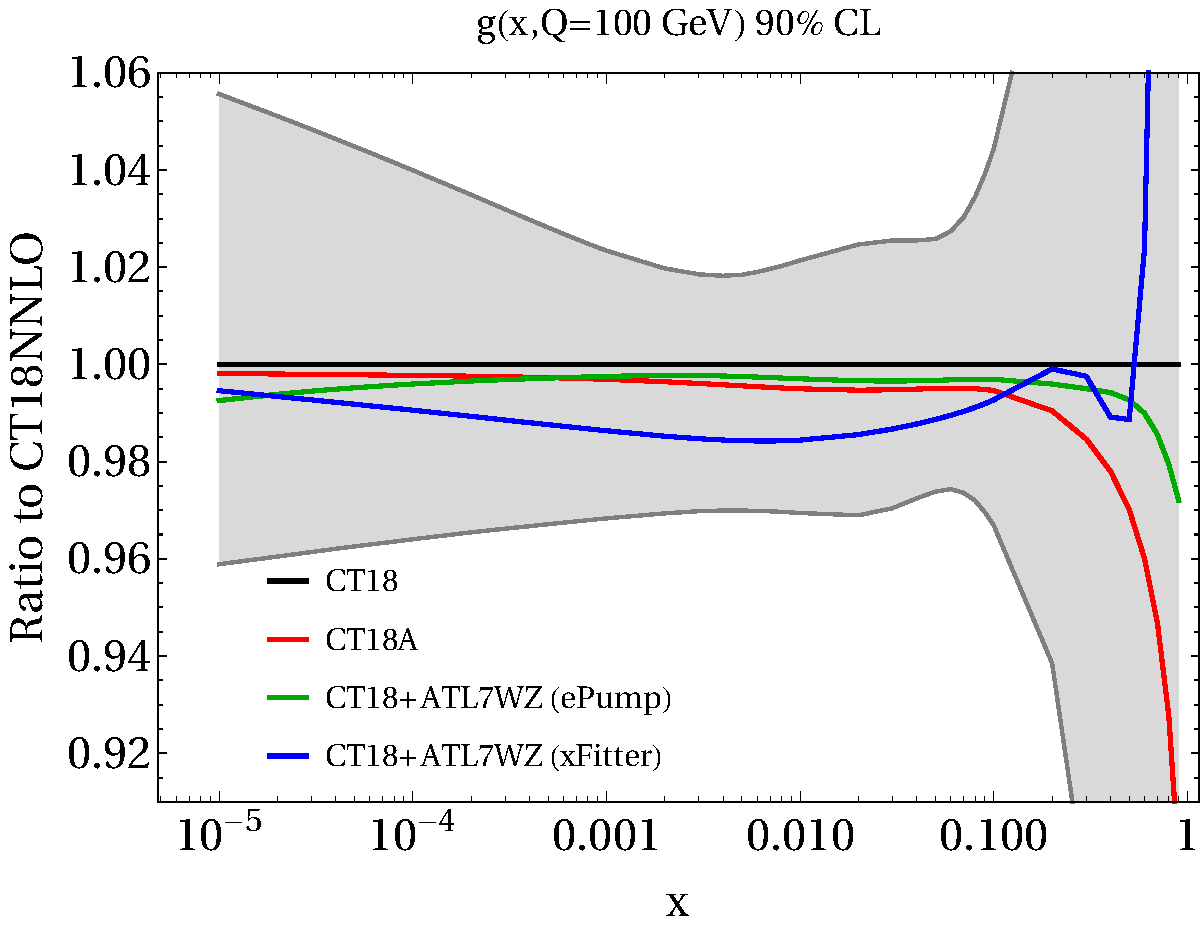
\includegraphics[width=0.45\textwidth]{fig/xFitter/CT18_ATL7WZ_xFitter_ePump_gluon_100GeV_2nd.pdf}
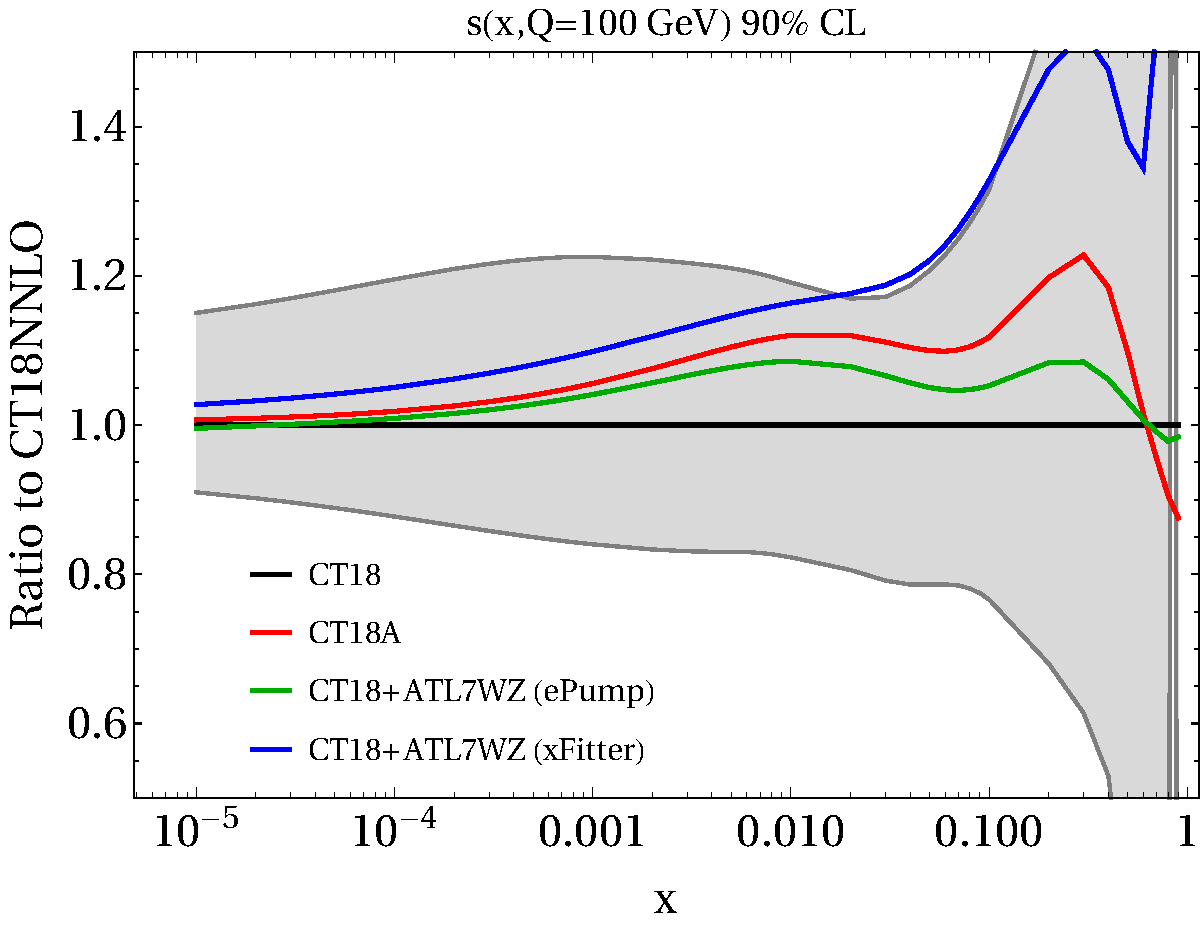
\includegraphics[width=0.45\textwidth]{fig/xFitter/CT18_ATL7WZ_xFitter_ePump_strange_100eV_2nd.pdf}
\caption{Gluon and strangeness PDFs at $Q=100$ GeV  for the CT18 (at 90\% C.L.) and CT18A global fits, compared with the respective central PDFs obtained by \texttt{ePump} dynamical-tolerance updating and the \texttt{xFitter} profiling of the CT18 PDFs by the ATLAS 7 TeV $W/Z$-production data. 
The \texttt{xFitter}-profiled PDFs are obtained with $T=1.645$ and include the diagonal second-order terms.
    }\label{fig:epxf-strange}
\end{figure}

{\bf Impact of the ATLAS $W/Z$ data.}
Here, we use the Hessian-profiling method of \texttt{xFitter}, as well as \texttt{ePump} updating, to explore the impact of the ATLAS 7 TeV inclusive $W/Z$-production data (Expt.~ID=248, \cite{Aaboud:2016btc})
on several PDF sets. The change in the total $\chi^{2}$ values before and after profiling/updating with the ATLAS 7 TeV $Z/W$-production data
is presented in Table~\ref{tab:chi2} for each PDF set. 
First, we explore all 7 measurements, having a total of $N_\textit{pt}=61$ data points: $W^{+}$, $W^{-}$, neutral current DY in the low-mass, $Z$-peak, and high-mass regions
for the central and forward selections. In this case, we can directly compare with the ATLAS \cite{Aaboud:2016btc} and MMHT \cite{Thorne:2019mpt} analyses. 
As a second case, we take only the 3 most precise measurements, {\it i.e.}, the $W^{+},\, W^{-}$, and $Z$-peak DY data for the central selection, with $N_{\textit{pt}}=34$ data points in total,
which are included in the NNPDF3.1 \cite{Ball:2017nwa} and CT18A(Z) global analyses. The comparison of the fitted $\chi^2/N_{\textit{pt}}$ values for these data in CT18A(Z), NNPDF3.1 and
MMHT can be found in Sec.~\ref{sec:CT18Z_qual}.

Table~\ref{tab:chi2} shows that the $\chi^{2}$ values of CT14, before and after \texttt{xFitter} profiling, agree well with the results presented in Ref.~\cite{Aaboud:2016btc}.
Here, we should apply the tolerance $T=1.645$ in \texttt{xFitter} as the CT PDFs are defined according to a 90\%
C.L.~\cite{Dulat:2015mca,Hou:2016nqm}.
%\cite{Tung:2006tb,Lai:2007dq,Nadolsky:2008zw,Lai:2010nw,Gao:2013xoa,Dulat:2015mca,Hou:2016nqm}. 
As shown in Ref.~\cite{Hou:2019gfw}, the same results can be reproduced by the \texttt{ePump}
code when the tolerance is set to $T\! =\! 1.645$. However, as clearly discussed in~\cite{Hou:2019gfw}, setting $T=1.645$ in the \texttt{ePump} calculation for the CT PDFs is equivalent to
assigning a very large weight (about $100/1.645^2$) to the new data set included in the fit.
\texttt{xFitter} profiling therefore generally overestimates the impact of new data sets when using the CT PDFs.
Meanwhile, a universal tolerance value ($T=1.645$) is not able to capture the constraints of Tier-2 penalty to determine the CT PDF error sets.
An appropriate way to update an existing CT PDF set with the
inclusion of any new experimental data is to adopt a dynamical tolerance.
%, with the specific value dependent on the corresponding direction of the PDF eigenvector~\cite{Hou:2019gfw}.
As such, \texttt{xFitter} profiling yields a smaller $\chi^2$ value (63) than
does~\texttt{ePump} updating with a dynamical tolerance (144), as can be seen by comparing the rightmost entries in the last row of Table~\ref{tab:chi2}.
This conclusion also holds when using~\texttt{xFitter} profiling with the MMHT~\cite{Harland-Lang:2014zoa} and PDF4LHC15~\cite{Butterworth:2015oua} PDFs.

The $\chi^2$ value of the 34 highest-precision ATLAS 7 TeV $W/Z$-production data points is found to be $\chi^2\!=\!87.6$ in the CT18A global fit, cf.~Table~\ref{tab:CMN}.
%Recall that CT18A is a global fit result after adding the ATLAS 7 TeV $W/Z$-production data to the original CT18 data set.   
To this we compare the corresponding value found using \texttt{ePump} updating with dynamical tolerance, for which we obtain $\chi^2\!=\!144$, as reported in Table~\ref{tab:chi2}.
This value includes two distinct contributions, $\chi^2_1=104$ from the difference between theory and data of the ATLAS 7 TeV $W/Z$-production itself, as well as from the quadrature sum $\chi^2_2=\sum_\alpha \lambda_{\alpha,\rm{th}}^2=40$ of theoretical nuisance parameters, which can be interpreted as the increase in $\chi^2$ of the other (``prior'') data sets included in the CT18 fit. 
The large increase in $\chi^2_2$, after \texttt{ePump} updating,  indicates the presence of some tensions between the ATLAS 7 TeV $W/Z$-production
data and the prior data sets, such as the CCFR/NuTeV SIDIS dimuon data~\cite{Hou:2019gfw}, cf.~Fig.~\ref{fig:lm_wht}.

The differences between the $\chi^2$ values in CT18A (87.6) and from \texttt{ePump} updating with a dynamical tolerance (104) indicate the breakdown of the linear approximation used
in the Hessian-updating method, when applied to this case. The breakdown can be confirmed by examining the updated central PDF set. In Fig.~\ref{fig:epxf-strange}, we show the gluon and strangeness
PDFs at $Q=100$ GeV for the CT18 (with 90\% C.L.~error) and CT18A global fits, compared with \texttt{ePump} dynamical-tolerance updating and \texttt{xFitter} profiling of CT18 with the ATLAS 7 TeV $W/Z$-production data.
%
%Here we have dropped the second-order terms in the PDF shifts of \texttt{xFitter} profiling in order to compare it with \texttt{ePump} updating on the same bases. 
%
As compared to the CT18 PDFs, we see that the updated $g$ and $s$ PDFs from the \texttt{ePump} program are similar to the CT18A PDFs, although with somewhat smaller shifts in the data-sensitive range, $10^{-3}\! <\! x\! <\! 10^{-1}$. In contrast, the default \texttt{xFitter} profiling produces a much larger shift in both $g$ and $s$ PDFs, than the
CT18A global fit.  As a result, \texttt{xFitter} profiling produces a too large change in the $s$-PDF, so that its central prediction touches the upper error band of CT18 at $x\! >\! 0.02$. 
We have found similar features in the comparison of other flavor PDFs. Namely, the default \texttt{xFitter} program generally overestimates the impact of new data sets in updating the
existing PDFs~\cite{Hou:2019gfw}. 

\begin{figure}[bhtp]
\begin{center}
%\includegraphics[width=0.46\textwidth]{figures/wplus.pdf}
%\includegraphics[width=0.46\textwidth]{figures/wminus.pdf}
%\includegraphics[width=0.46\textwidth]{figures/zypeak.pdf}
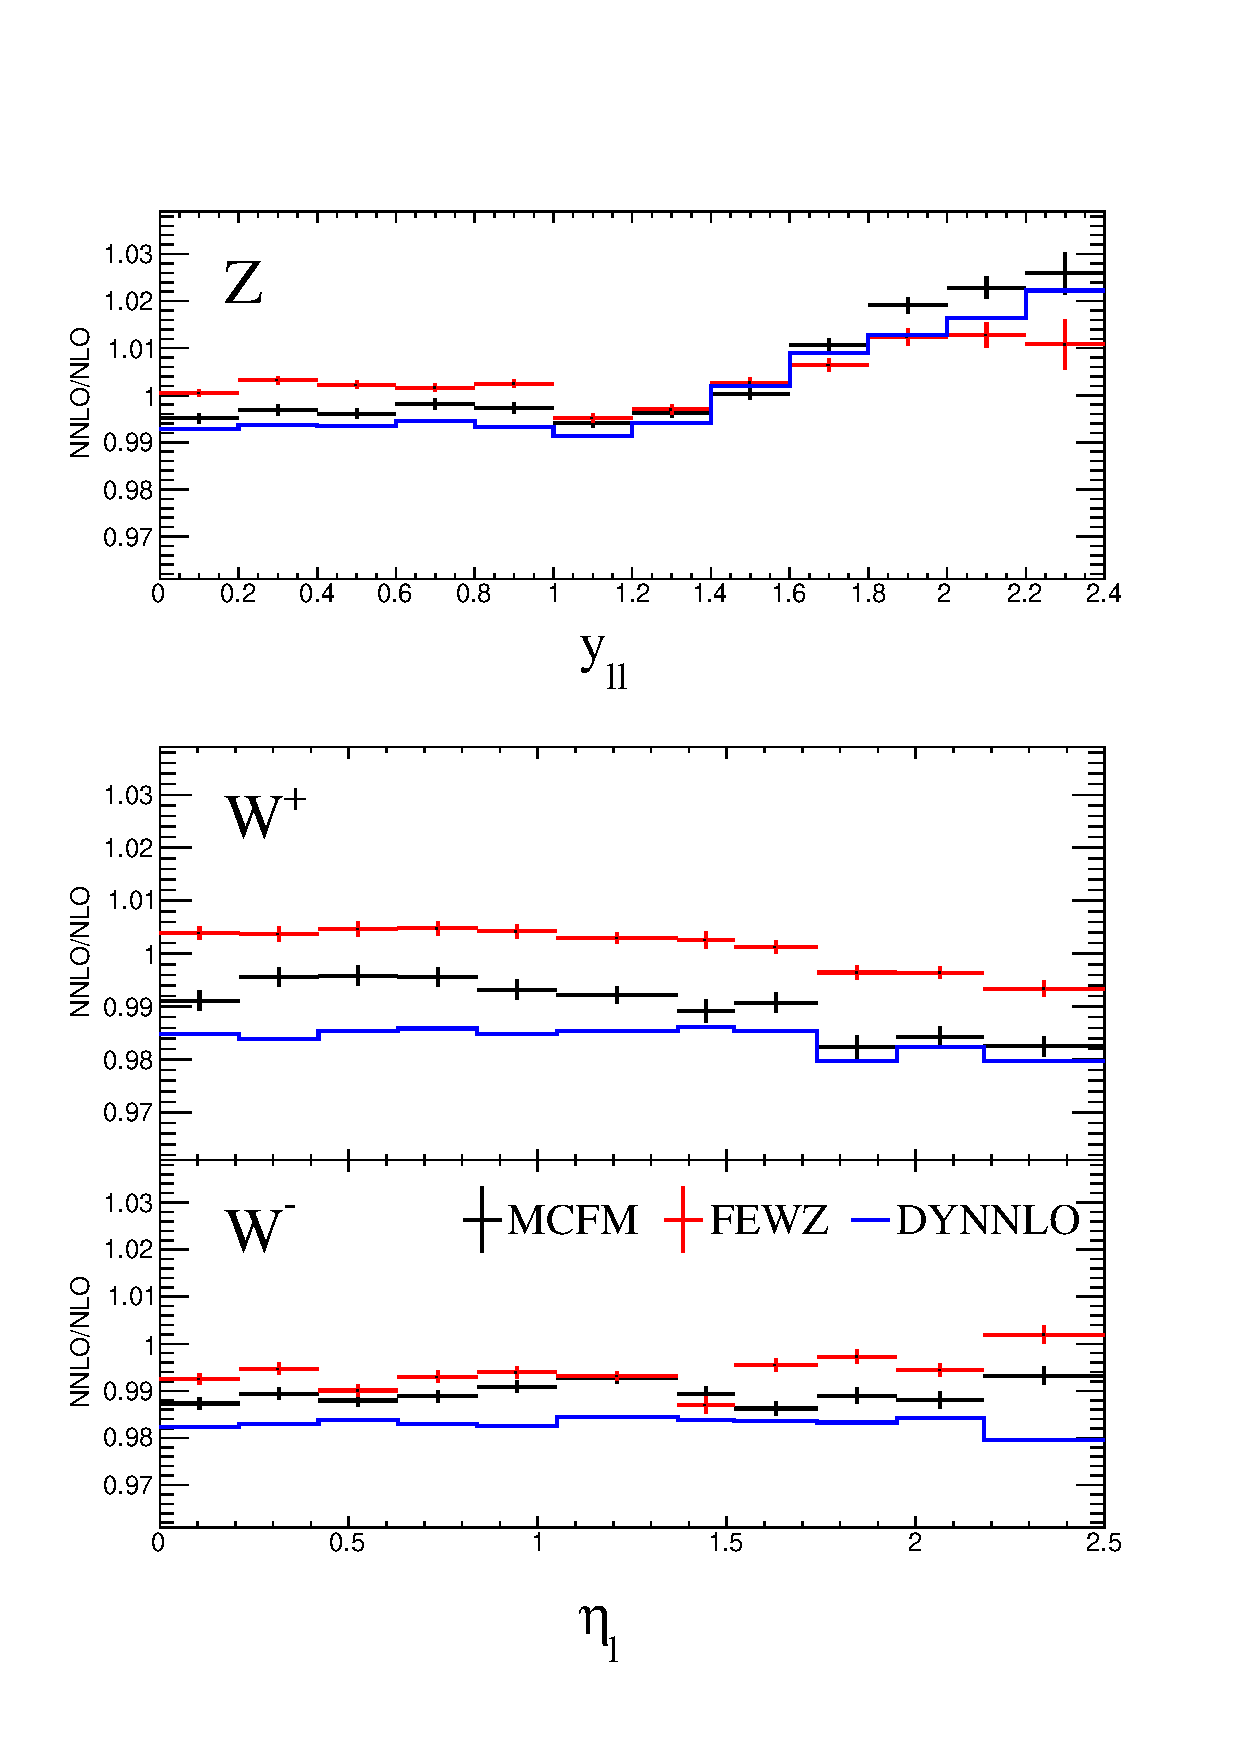
\includegraphics[width=0.8\textwidth]{fig/fig2/ATL7WZ_KF.pdf}
\caption{The comparison of $K$-factors for the ATLAS 7 TeV $W/Z$ data calculated with \texttt{DYNNLO}, \texttt{FEWZ} and \texttt{MCFM}. The error bars indicate the theoretical Monte-Carlo uncertainties. The \texttt{DYNNLO} curves are extracted from \texttt{xFitter} and include NLO EW corrections.} 
\label{fig:Kfactors}
\end{center}
\end{figure}

\begin{table}
\caption{
The $\chi^2$ values for the ATLAS 7 TeV $W/Z$-production data (with 34 data points in total), before and after the \texttt{xFitter} profiling and the \texttt{ePump} dynamical-tolerance updating, with various NNLO predictions. (See the text for details.)
We do not update  CT18A(Z) fits to avoid 
double-counting the impact of the ATLAS 7 TeV $W/Z$-production data.
}
\label{tab:chi2Kfactors}
\begin{tabular}{c|c|c|c|c|c|c}
\hline
 &  \multicolumn{2}{c|}{\texttt{DYNNLO}} &    \multicolumn{2}{c|}{\texttt{MCFM}} &  \multicolumn{2}{c}{\texttt{FEWZ}}  \\
\hline
\multicolumn{7}{c}{\texttt{xFitter} profiling}\\
\hline
PDF & before & after   & before & after   & before & after \\
\hline
CT18 & 294 & 63    &  277 & 65  & 225  &  62   \\
CT18A & 87  & --   & 92   & --  & 109  & --    \\
CT18Z & 88 &   --  &  94  & --  & 109  &  --  \\
\hline
\multicolumn{7}{c}{\texttt{ePump} dynamic-tolerance updating}\\
\hline
CT18 & 289 & 144   &  273  & 144    & 223   & 135    \\
CT18A & 87 & --   &  91  & --  &  109 &  --  \\
CT18Z & 88 &   --   &  94  & --  &  109 & --  \\
\hline
\end{tabular}
\end{table}

{\bf Comparison of different NNLO predictions.}
In addition to the studies described above, we have also used the \texttt{xFitter} and \texttt{ePump} frameworks
to examine aspects of the theory calculations for the ATLAS 7 TeV $W/Z$ data.
%
In the CT18A(Z) global fits, the NNLO predictions for these measurements were calculated using NNLO/NLO $K$-factors combined with NLO  \texttt{APPLGrid} predictions.  Specifically, the $K$-factors used in our CT18A(Z) fits were 
directly extracted from \texttt{xFitter}, where they were calculated with the \texttt{DYNNLO} code~\cite{Catani:2007vq,Catani:2009sm}. 
It was noted by the ATLAS Collaboration in 
Ref.~\cite{Aaboud:2016btc} that the integrated fiducial  $Z$ , $W^{+}$ and $W^{-}$ cross sections predicted by the NNLO codes 
\texttt{FEWZ} \cite{Gavin:2010az,Gavin:2012sy,Li:2012wna} and \texttt{DYNNLO} \cite{Catani:2007vq,Catani:2009sm} differ 
by about 0.2\%, 1.2\% and 0.7\%, respectively.
Fig.~\ref{fig:Kfactors} shows a slightly larger difference, since the \texttt{DYNNLO} curves include the NLO EW corrections, while other two do not.


Next, we wish to compare various NNLO predictions for differential cross section measurements of the ATLAS 7 TeV $W/Z$-production data.  
First, we verified that the NLO predictions agree, within 0.2\%, among  \texttt{DYNNLO},  \texttt{MCFM}~\cite{Boughezal:2016wmq,MCFM8} 
and \texttt{FEWZ}, which reflects the fact that all three codes adopt the dipole formalism \cite{Catani:1996jh,Catani:1996vz} in the NLO calculations. 
Since the NNLO predictions can be expressed as the NLO predictions multiplied by their $K$-factors, we compare in Fig. \ref{fig:Kfactors} the $K$-factors obtained from each code,
for every ATLAS 7 TeV $W/Z$-production data point (with 34 data points in total).
It can be seen that the differences among the three $K$-factors vary as a function of the $Z$-boson rapidity, or the rapidity of the charged lepton from the $W$-boson decay. 
These differences can be sizable, $\gtrsim\!1\%$, as compared to the typically sub-percent statistical uncertainty found in the ATLAS 7 TeV $W/Z$ data.  
We also find that the predictions of \texttt{MCFM} generally lie between those of \texttt{DYNNLO} and \texttt{FEWZ}. This difference can be understood as a consequence
of the the different NNLO techniques: \texttt{FEWZ} adopts sector decomposition \cite{Binoth:2000ps,Anastasiou:2003gr,Anastasiou:2005qj}, while \texttt{DYNNLO} and \texttt{MCFM}
are based on transverse-momentum ($q_T$) \cite{Catani:2007vq,Catani:2009sm} and $N$-jettiness ($\mathcal{T}_N$) \cite{Boughezal:2016wmq} subtractions, respectively. 
%The NNLO cross sections calculated with phase space-slicing methods converge in the limit when the phase cuts approach 0, {\it i.e.}, $q_T^{\textrm{cut}}\to0$ or $\mathcal{T}_N^{\textrm{cut}}\to0$.
% The 1\% discrepancy can be ascribed to the nonzero phase cuts in our practical calculations. 

It is also useful to investigate the dependence of the ATLAS 7 TeV $W/Z$ fit quality on the specific choice of NNLO calculation scheme. 
Table~\ref{tab:chi2Kfactors} summarizes the findings of such a study. 
After CT18 PDFs are updated using \texttt{ePump} with the ATLAS 7 TeV $W/Z$ data, we find that the final $\chi^2$ value for the ATLAS $W/Z$ data set
is equal to 144, 144, and 135 units when theory is predicted by the \texttt{DYNNLO}, \texttt{MCFM} and \texttt{FEWZ} NNLO calculations, respectively. 
Hence, we conclude that these three NNLO calculations lead to fits of similar quality for the ATLAS 7 TeV $W/Z$ data.
A similar conclusion also holds when using the \texttt{xFitter} framework, with the final $\chi^2$ values being 63, 65 and 62 units, respectively.
To recap, the default \texttt{xFitter} profiling (with tolerance $T\! =\! 1.645$ ) overestimates the impact of the
ATLAS 7 TeV $W/Z$ data when updating the CT18 PDFs, explaining why it yields a smaller $\chi^2$ value than \texttt{ePump} updating. We also confirm that the updated PDFs by the three $K$-factors differ slightly, but the difference is negligible compared with the same systematical shifts due to the experimental uncertainties.  
In conclusion, the NNLO theoretical predictions for the ATLAS 7 TeV $W/Z$ data by \texttt{DYNNLO}, \texttt{MCFM} and \texttt{FEWZ}  show perceptible differences when using the same PDF set. On the other hand, after the PDFs are updated by either \texttt{ePump} and \texttt{xFitter}, the final $\chi^2$ and PDFs show minor differences among the three codes.